% ============================================================
%  Cerebral Autoregulation — Three-Panel Figure (Fig. 92.1)
%  Panels: A) CBF vs CPP   B) ICP vs CPP   C) MAP vs CPP
%
%  Mathematical relationship:  CPP = MAP − ICP
%  Therefore:                  MAP = CPP + ICP
%
%  Panel C coordinates are derived by adding the ICP value at
%  each CPP landmark to that CPP value, making all three panels
%  internally consistent.
%
%  Requires: pdflatex + pgfplots (tikz)
%  Build:    pdflatex cerebral_autoregulation.tex
% ============================================================
\documentclass[12pt]{article}
\usepackage{tikz}
\usepackage{pgfplots}
\pgfplotsset{compat=1.18}
\usepackage[margin=1.8cm]{geometry}
\usepackage{xcolor}

% ── Colour palette ────────────────────────────────────────────
\definecolor{autoreg}{RGB}{255,255,153}   % soft yellow  – autoregulation zone
\definecolor{icpcol} {RGB}{173,216,230}   % light blue   – ICP normal band
\definecolor{danger} {RGB}{255,200,200}   % light red    – dysregulation zones
\definecolor{mapcol} {RGB}{200,230,200}   % soft green   – MAP normal range

\begin{document}
\begin{figure}[p]
\centering
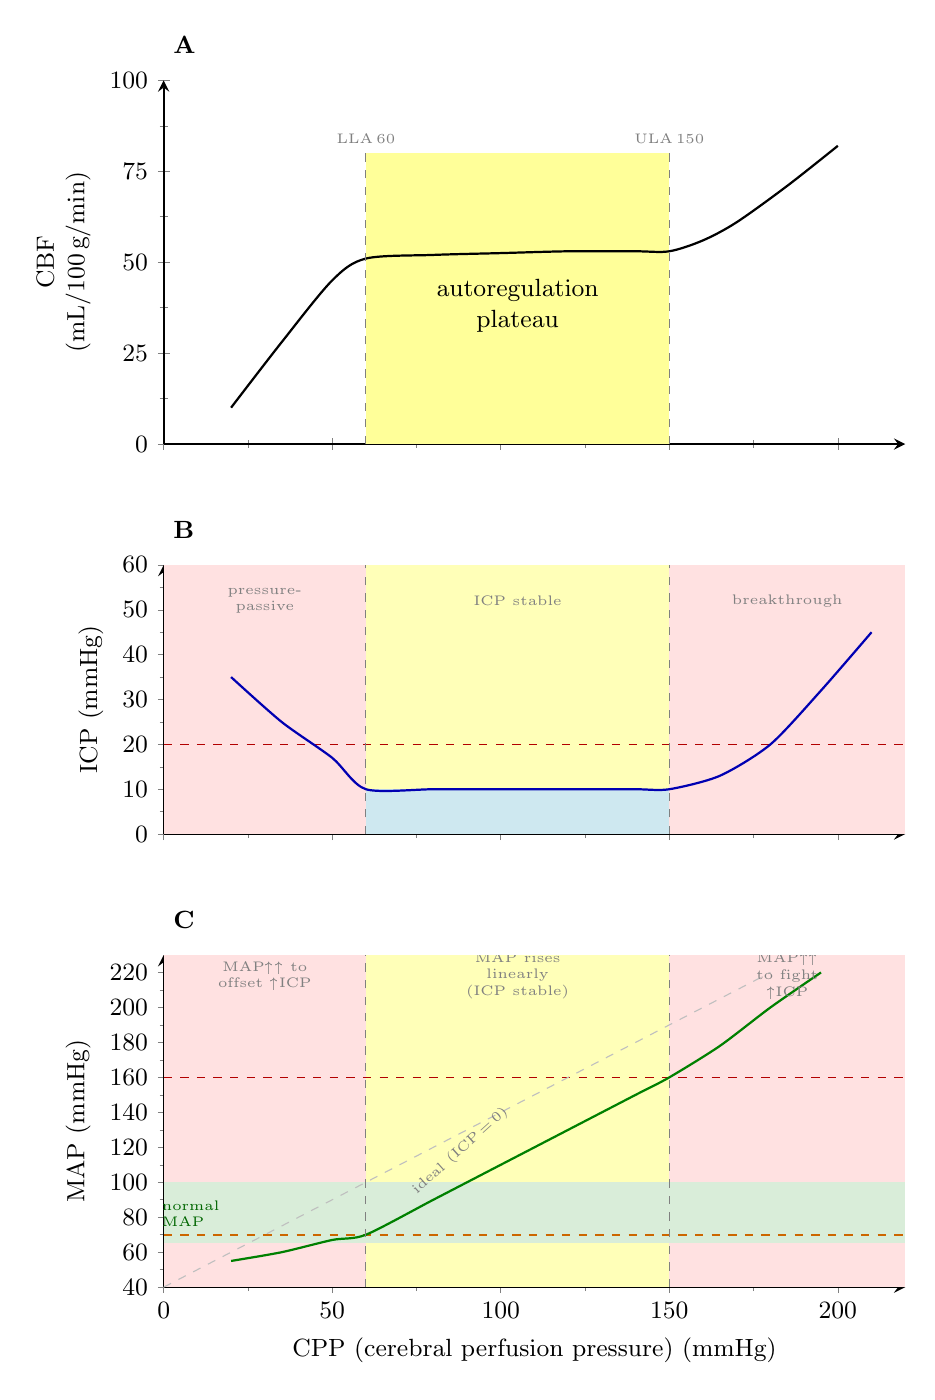
\begin{tikzpicture}

  % ==============================================================
  %  PANEL A — CBF vs CPP  (top)
  % ==============================================================
  \begin{axis}[
    name        = cbfaxis,
    width  = 11cm,
    height =  6.2cm,
    xmin=0, xmax=220,
    ymin=0, ymax=100,
    xtick       = {0,50,100,150,200},
    xticklabels = {},
    ytick       = {0,25,50,75,100},
    minor xtick = {25,75,125,175},
    minor ytick = {12.5,37.5,62.5,87.5},
    ylabel       = {CBF\\(mL/100\,g/min)},
    ylabel style = {align=center, font=\small},
    tick label style = {font=\small},
    axis lines   = left,
    axis line style = {thick},
    title        = {\textbf{A}},
    title style  = {at={(0,1)}, anchor=south west, font=\bfseries\small},
    clip         = true,
  ]
    \fill[autoreg] (axis cs:60,0) rectangle (axis cs:150,80);
    \node[font=\small, align=center] at (axis cs:105,38)
      {autoregulation\\ plateau};

    \addplot[black, thick, smooth, tension=0.5] coordinates {
      (20,  10)(35,  28)(50,  45)(60,  51)(80,  52)
      (100, 52.5)(120, 53)(140, 53)(150, 53)
      (160, 56)(170, 61)(185, 71)(200, 82)
    };

    \draw[dashed, gray, thin] (axis cs:60,0)  -- (axis cs:60,80);
    \draw[dashed, gray, thin] (axis cs:150,0) -- (axis cs:150,80);
    \node[font=\tiny, gray, above] at (axis cs:60,80)  {LLA\,60};
    \node[font=\tiny, gray, above] at (axis cs:150,80) {ULA\,150};
  \end{axis}

  % ==============================================================
  %  PANEL B — ICP vs CPP  (middle)
  %
  %  ICP landmarks (also used to compute Panel C):
  %   (CPP, ICP): (20,35)(35,25)(50,17)(60,10)(80,10)(100,10)
  %               (120,10)(140,10)(150,10)(165,13)(180,20)(195,32)(210,45)
  % ==============================================================
  \begin{axis}[
    name        = icpaxis,
    at          = {(cbfaxis.below south west)},
    anchor      = above north west,
    yshift      = -0.55cm,
    width  = 11cm,
    height =  5cm,
    xmin=0, xmax=220,
    ymin=0, ymax=60,
    xtick       = {0,50,100,150,200},
    xticklabels = {},
    ytick       = {0,10,20,30,40,50,60},
    minor xtick = {25,75,125,175},
    minor ytick = {5,15,25,35,45,55},
    ylabel       = {ICP (mmHg)},
    ylabel style = {align=center, font=\small},
    tick label style = {font=\small},
    axis lines   = left,
    axis line style = {thick},
    title        = {\textbf{B}},
    title style  = {at={(0,1)}, anchor=south west, font=\bfseries\small},
    clip         = true,
  ]
    \fill[danger!55]  (axis cs:0,0)   rectangle (axis cs:60,60);
    \fill[autoreg!70] (axis cs:60,0)  rectangle (axis cs:150,60);
    \fill[danger!55]  (axis cs:150,0) rectangle (axis cs:220,60);
    \fill[icpcol!60]  (axis cs:60,0)  rectangle (axis cs:150,10);

    \draw[red!70!black, dashed, semithick]
      (axis cs:0,20) -- (axis cs:220,20)
      node[right, font=\tiny, red!70!black] {critical ICP\,20};

    \addplot[blue!70!black, thick, smooth, tension=0.45] coordinates {
      (20,35)(35,25)(50,17)(60,10)(80,10)(100,10)
      (120,10)(140,10)(150,10)(165,13)(180,20)(195,32)(210,45)
    };

    \draw[dashed, gray, thin] (axis cs:60,0)  -- (axis cs:60,60);
    \draw[dashed, gray, thin] (axis cs:150,0) -- (axis cs:150,60);

    \node[font=\tiny, align=center, gray] at (axis cs:30, 52)
      {pressure-\\ passive};
    \node[font=\tiny, align=center, gray] at (axis cs:105,52)
      {ICP stable};
    \node[font=\tiny, align=center, gray] at (axis cs:185,52)
      {breakthrough};
  \end{axis}

  % ==============================================================
  %  PANEL C — MAP vs CPP  (bottom)
  %
  %  MAP = CPP + ICP  (computed from Panel B landmarks):
  %   (20,55)(35,60)(50,67)(60,70)(80,90)(100,110)(120,130)
  %   (140,150)(150,160)(165,178)(180,200)(195,220 clipped)
  %
  %  Within the plateau ICP ≈ 10 mmHg = const →
  %    slope dMAP/dCPP = 1  (linear, offset by 10)
  %  Outside the plateau rising ICP steepens the slope:
  %    dMAP/dCPP = 1 + dICP/dCPP  > 1
  % ==============================================================
  \begin{axis}[
    name        = mapaxis,
    at          = {(icpaxis.below south west)},
    anchor      = above north west,
    yshift      = -0.55cm,
    width  = 11cm,
    height =  5.8cm,
    xmin=0, xmax=220,
    ymin=40, ymax=230,
    xtick       = {0,50,100,150,200},
    ytick       = {40,60,80,100,120,140,160,180,200,220},
    minor xtick = {25,75,125,175},
    minor ytick = {50,70,90,110,130,150,170,190,210},
    xlabel       = {CPP (cerebral perfusion pressure) (mmHg)},
    ylabel       = {MAP (mmHg)},
    xlabel style = {font=\small},
    ylabel style = {align=center, font=\small},
    tick label style = {font=\small},
    axis lines   = left,
    axis line style = {thick},
    title        = {\textbf{C}},
    title style  = {at={(0,1)}, anchor=south west, font=\bfseries\small},
    clip         = true,
  ]
    % Zone backgrounds
    \fill[danger!55]  (axis cs:0,40)   rectangle (axis cs:60,230);
    \fill[autoreg!70] (axis cs:60,40)  rectangle (axis cs:150,230);
    \fill[danger!55]  (axis cs:150,40) rectangle (axis cs:220,230);

    % Normal MAP band 65–100 mmHg
    \fill[mapcol!70] (axis cs:0,65) rectangle (axis cs:220,100);
    \node[font=\tiny, green!40!black, align=left]
      at (axis cs:8,82) {normal\\ MAP};

    % MAP = 70 threshold  (LLA: CPP 60 + ICP 10)
    \draw[orange!80!black, dashed, semithick]
      (axis cs:0,70) -- (axis cs:220,70)
      node[right, font=\tiny, orange!80!black] {MAP\,70};

    % MAP = 160 threshold  (ULA: CPP 150 + ICP 10)
    \draw[red!70!black, dashed, semithick]
      (axis cs:0,160) -- (axis cs:220,160)
      node[right, font=\tiny, red!70!black] {MAP\,160};

    % Theoretical reference: MAP = CPP (ICP = 0, slope 1 through origin)
    \addplot[gray!50, thin, dashed] coordinates {(0,40)(180,220)};
    \node[font=\tiny, gray, rotate=42] at (axis cs:88,118) {ideal (ICP\,=\,0)};

    % MAP curve  (MAP = CPP + ICP)
    \addplot[green!50!black, thick, smooth, tension=0.45] coordinates {
      (20,  55)
      (35,  60)
      (50,  67)
      (60,  70)
      (80,  90)
      (100,110)
      (120,130)
      (140,150)
      (150,160)
      (165,178)
      (180,200)
      (195,220)
    };

    % Boundary lines
    \draw[dashed, gray, thin] (axis cs:60,40)  -- (axis cs:60,230);
    \draw[dashed, gray, thin] (axis cs:150,40) -- (axis cs:150,230);

    % Zone annotations
    \node[font=\tiny, align=center, gray] at (axis cs:30, 218)
      {MAP↑↑ to\\ offset ↑ICP};
    \node[font=\tiny, align=center, gray] at (axis cs:105,218)
      {MAP rises\\ linearly\\ (ICP stable)};
    \node[font=\tiny, align=center, gray] at (axis cs:185,218)
      {MAP↑↑\\ to fight\\ ↑ICP};

  \end{axis}

\end{tikzpicture}

\medskip
\noindent\textbf{Fig.\,92.1\quad Cerebral autoregulation: CBF, ICP, and MAP as functions of CPP.}\\[3pt]
\small
All three panels share the same x-axis (CPP 0–220\,mmHg) and are coupled by the identity
\(\mathbf{CPP = MAP - ICP}\).
Vertical dashed lines mark the lower (LLA\,=\,60\,mmHg) and upper (ULA\,=\,150\,mmHg)
limits of autoregulation (yellow zone).
\textbf{A.}~CBF is pressure-independent across the plateau.
\textbf{B.}~ICP \(\approx\)10\,mmHg within the plateau; it rises steeply below the LLA
(exhausted vasodilatory reserve) and above the ULA (breakthrough hyperperfusion /
vasogenic oedema). Dashed red line = critical ICP of 20\,mmHg.
\textbf{C.}~MAP\,=\,CPP\,+\,ICP: within the plateau ICP is constant so MAP rises linearly
with CPP at slope\,=\,1 (green curve); outside the plateau the rising ICP forces MAP to
increase disproportionately to sustain the same CPP (slope\,\(>\)\,1).
Orange dashed line = minimum MAP target at the LLA (\(\approx\)70\,mmHg);
red dashed line = ULA MAP ceiling (\(\approx\)160\,mmHg).
Green band = normal MAP range (65–100\,mmHg).
The diagonal grey reference shows the theoretical MAP–CPP line if ICP were zero.

\end{figure}
\end{document}
